\documentclass{article}
\usepackage{verbatim}
\usepackage{tikz,times}
\usepackage[paperwidth=25cm,left=1cm,top=1cm]{geometry}
\usetikzlibrary{mindmap,backgrounds}
\pagestyle{empty}
\begin{document}
\centering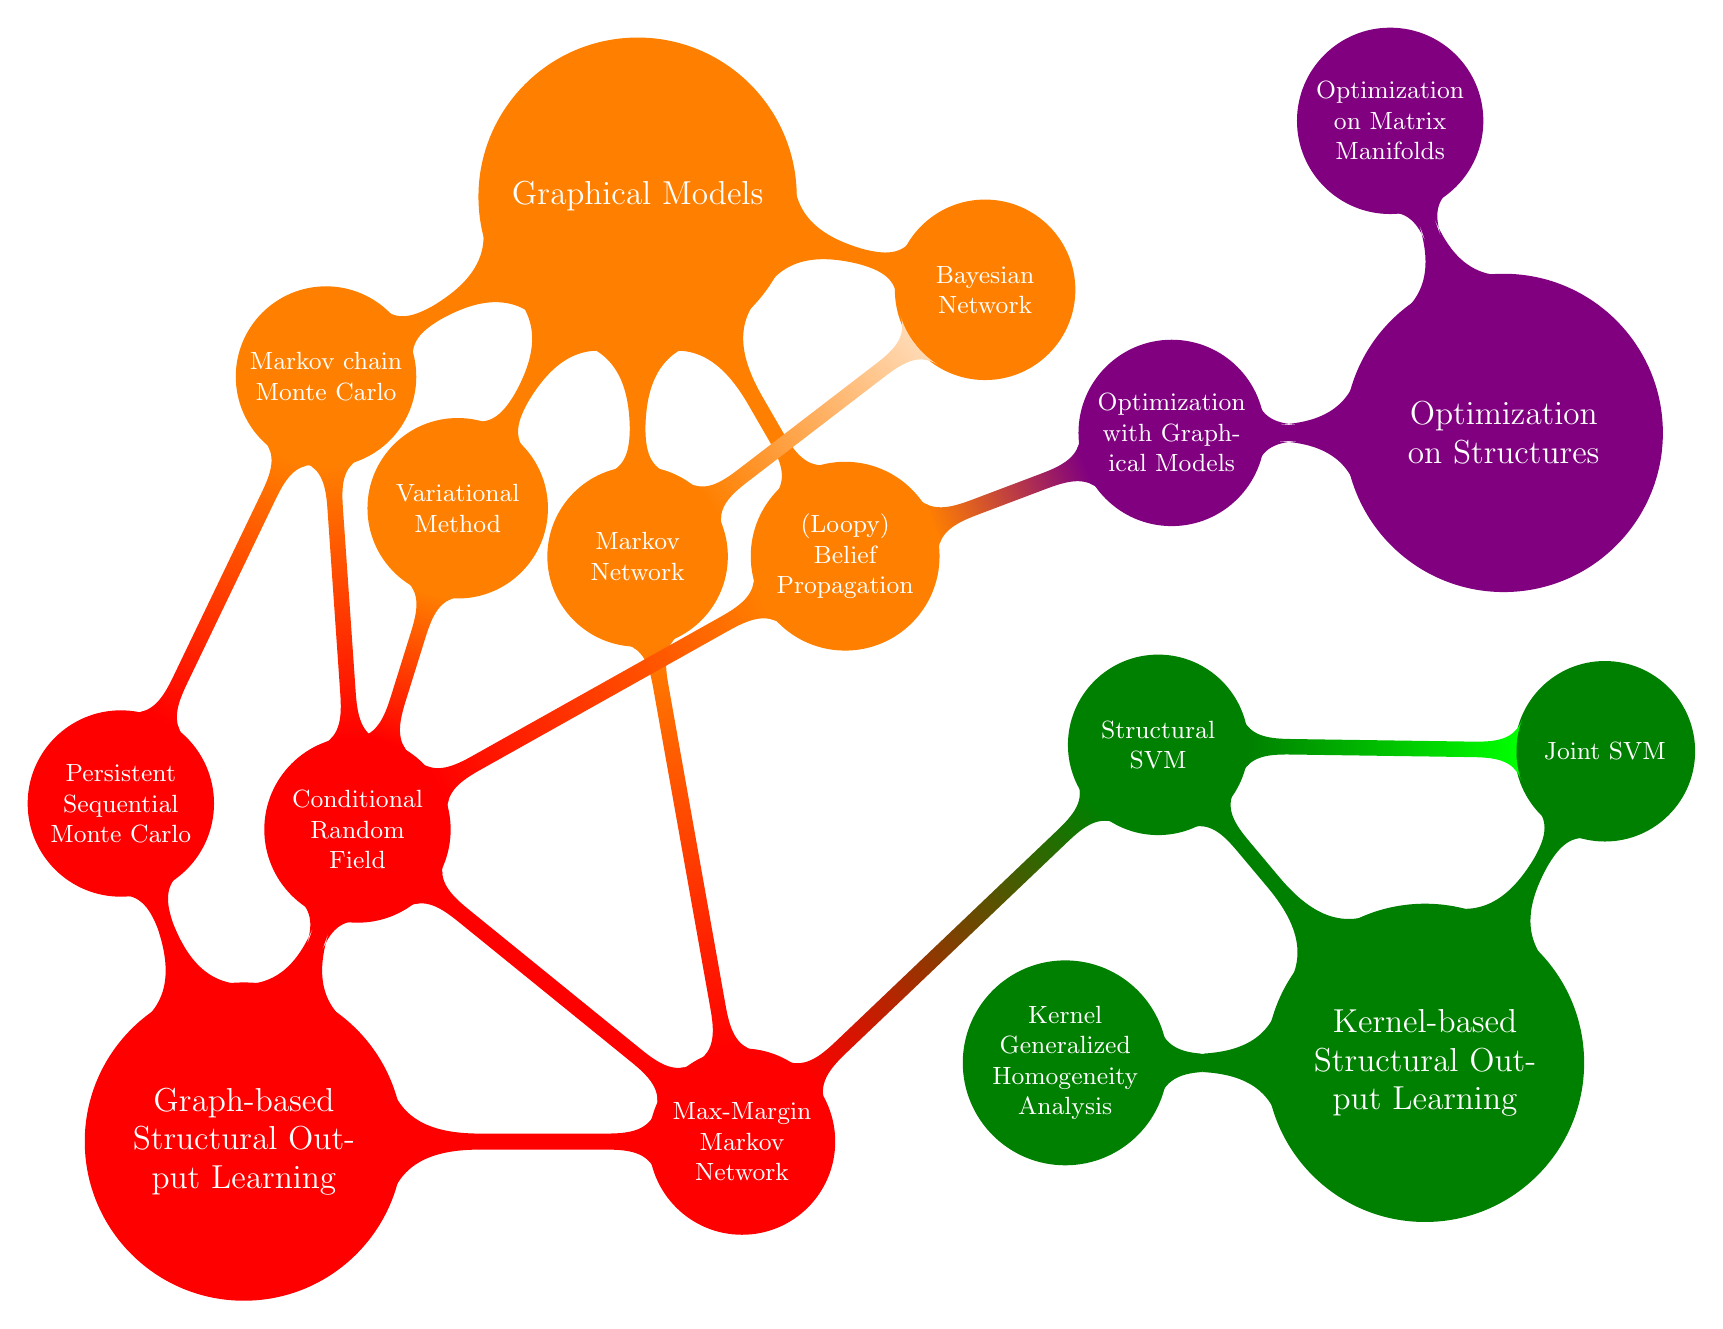
\begin{tikzpicture}[mindmap,
  level 1 concept/.append style={level distance=130,sibling angle=30},
  extra concept/.append style={color=blue!50,text=black}]

  % Applied area: computer science and its subfields

  \begin{scope}[mindmap, concept color=orange, text=white]
    \node [concept] {Graphical Models}[clockwise from=-5] 
	  child [grow=-15]{node [concept] (BN) {Bayesian Network}}
	  child [grow=-90]{node [concept] (MN) {Markov Network}}
	  child [grow=-60, level distance=150]{node [concept] (BP) {(Loopy) Belief Propagation}}
	  child [grow=-120]{node [concept] (VA) {Variational Method}}
	  child [grow=-150]{node [concept] (MCMC) {Markov chain Monte Carlo}};
  \end{scope}

  % Applied area: theoretical physics and its subfields

  \begin{scope}[mindmap, concept color=red,text=white]
    \node [concept] at (-5,-12) {Graph-based Structural Output Learning}
      child [grow=70, level distance=120] 
        {node [concept] (CRF) {Conditional Random Field}}
      child [grow=0, level distance=180]
        {node [concept] (M3N) {Max-Margin Markov Network}}
      child [grow=110] 
        {node [concept] (PSMC) {Persistent Sequential Monte Carlo}};
  \end{scope}

  % Applied area: biology and its subfields

  \begin{scope}[mindmap, concept color=green!50!black,text=white]
    \node [concept] at (10,-11) {Kernel-based Structural Output Learning} 
      child [grow=130, level distance=150] 
        {node [concept] (SSVM) {Structural SVM}}
      child [grow=60] 
        {node [concept] (JSVM) {Joint SVM}}
      child [grow=180] 
        {node [concept] (KGHA) {Kernel Generalized Homogeneity Analysis}};
  \end{scope}

  % Applied area: economics (one subfield)

  \begin{scope}[mindmap, concept color=violet, text=white]
    \node [concept] at (11,-3) {Optimization on Structures}
      child [grow=-180, level distance=120] 
        {node [concept] (MBP) {Optimization with Graphical Models}}
      child [grow=110, level distance=120] 
        {node [concept] (MAN) {Optimization on Matrix Manifolds}};

  \end{scope}

  % Researchers listed by their main specialization in mathematics

  % Connections of researchers to applied subfields

  %\begin{pgfonlayer}{background}
   % \draw [fill=black,circle connection bar]
	  \path (BN) to [circle connection bar switch color=from (orange!30!white) to (orange)] (MN);
      \path (M3N) to [circle connection bar switch color=from (red) to (orange)] (MN);
      \path (M3N) to [circle connection bar switch color=from (red) to (red)] (CRF);
	  \path (M3N) to [circle connection bar switch color=from (red) to (green!50!black)] (SSVM);     
	  \path (MBP) to [circle connection bar switch color=from (violet) to (orange)](BP); 
	  \path (JSVM) to [circle connection bar switch color=from (green!100!black) to (green!50!black)]  (SSVM);
	  \path (PSMC) to [circle connection bar switch color=from (red) to (orange)]  (MCMC); 
	  \path (CRF) to [circle connection bar switch color=from (red) to (orange)] (BP);
	  \path (CRF) to [circle connection bar switch color=from (red) to (orange)] (VA);
	  \path (CRF) to [circle connection bar switch color=from (red) to (orange)] (MCMC); 
 % \end{pgfonlayer}
\end{tikzpicture}
\end{document}
